\subsection{Size control: small ovals at half-length $1.53\,\la$}\label{sec:p3}
Four shapes ($b/a=2.5, 2.0, 1.6, 1.3$), $k=6$, 3 seeds each, at the size where circles are cleanest
(between the circles of $R=1.43$ and $1.72\,\la$). The geometric effect holds, with a sharp crossover in elongation:
\begin{table}[h]\centering\small
\caption{Small ovals (half-length $1.53\,\la$, 3 seeds) compared with circles of comparable size. Aspect = length / height.}\label{tab:p3}
\begin{tabular}{lcccccc}\toprule
cavity & aspect & sites & $q_b$ (site rule) & labels at wall after 1000 & criteria agree & $d^*/\la$\\\midrule
circle $R=1.43\,\la$ & 1 & 10 & 1.01--1.05 & 0.87--0.94 & 97--99\% & 0.19--0.20\\
oval $b/a=2.5$ & 1.17 & 10 & 1.07--1.11 & 0.82--0.86 & 97--98\% & 0.22--0.23\\
oval $b/a=2.0$ & 1.29 & 8--9 & 1.6--2.1 & 0.60--0.65 & 81--86\% & 0.29--0.31\\
oval $b/a=1.6$ & 1.5 & 13--14 & 3.3--3.5 & 0.37--0.40 & 72--74\% & 0.41\\
oval $b/a=1.3$ & 1.9 & 8--16 & 3.3--3.6 & 0.42--0.50 & 69--72\% & 0.49--0.50\\\bottomrule
\end{tabular}
\end{table}
At $b/a=2.5$ the oval is circle-like in every measure ($2k-2$ pinned sites, bulk $+1$, wall defects stay). At $b/a=2.0$
the structure is partly lost, and at $b/a\le1.6$ (still convex) it is gone. Same size, different shape, different
charge split: \textbf{the split is geometric.}

\subsection{A single number: the layer depth $d^*$}
Following B.~Loewe's suggestion: $c^*$ is where $Q(c)$ crosses $+1$ on its way to $k$, and $d^*$ the mean wall distance along
that level (circle: $R-c^*$). Normalised by $\la$ (by size, $d^*/R$ hardly changes in circles even when the layer degrades).
\begin{figure}[h]\centering
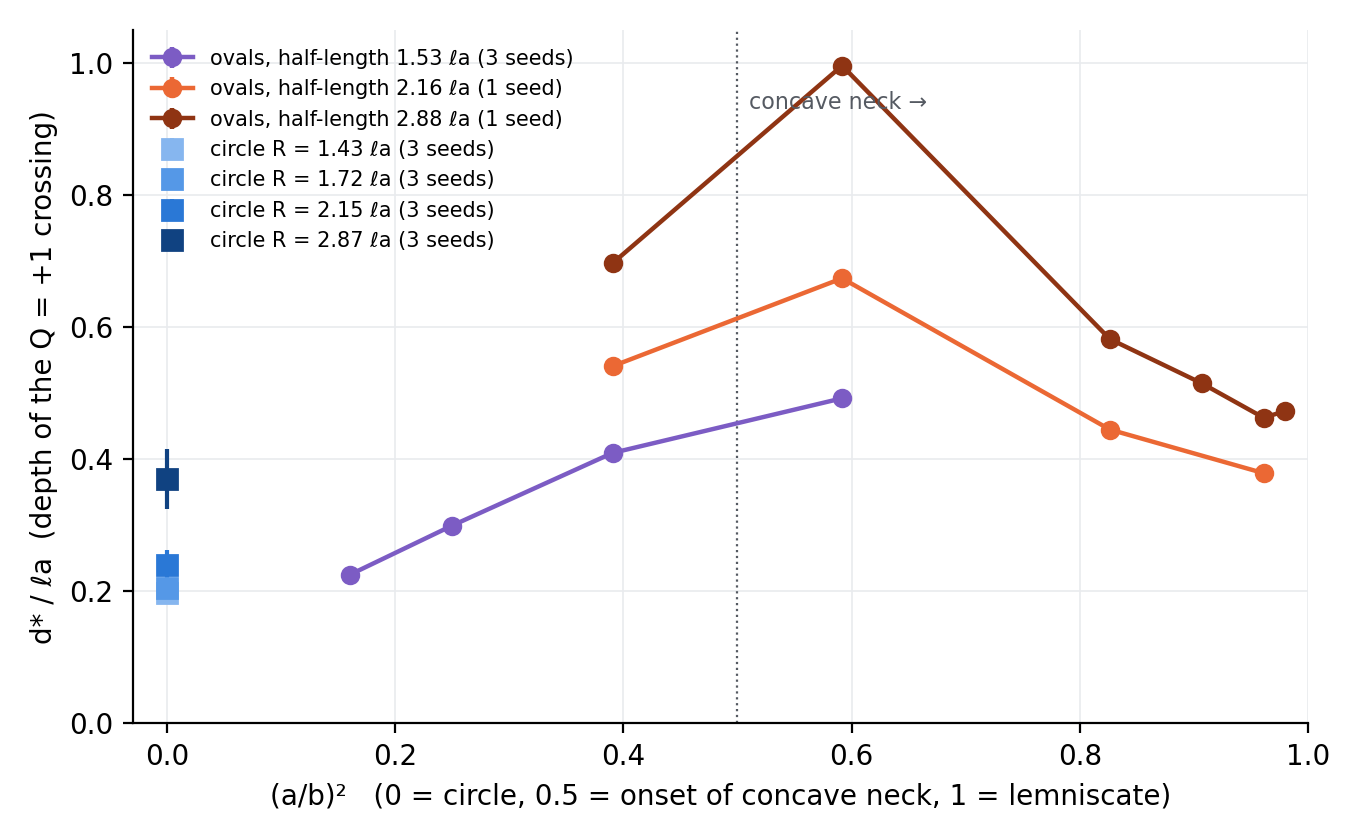
\includegraphics[width=0.82\textwidth]{figs/layer_depth.png}
\caption{Layer depth $d^*/\la$ versus elongation $(a/b)^2$ (0 circle, 0.5 onset of the concave neck, 1 lemniscate), $k=6$.
Circles 4.5--6 cells ($\approx0.2\,\la$) up to $R=2.15\,\la$. Small ovals rise from 0.23 to 0.50; larger ovals peak near
$b/a\approx1.3$.}\label{fig:dstar}
\end{figure}
See Fig.~\ref{fig:Qc} for the accumulated charge including the small ovals.

\subsection{Area fraction of the ``layer''}
Also following B.~Loewe: $f^*=A(c>c^*)/A_\mathrm{total}$, the fraction of the cavity between the $Q=+1$ level and the wall,
and the equivalent strip width $w_\mathrm{eff}=A(c>c^*)/P$. A true layer has a fixed width, so $f^*$ falls with cavity size
(circles: 0.26 at $1.43\,\la$, 0.20 at $2.15\,\la$); a charge distribution spread through the cavity gives a size-independent
$f^*$. Beyond $f^*=\frac12$ the ``layer'' would be larger than the bulk it surrounds.
\begin{figure}[h]\centering
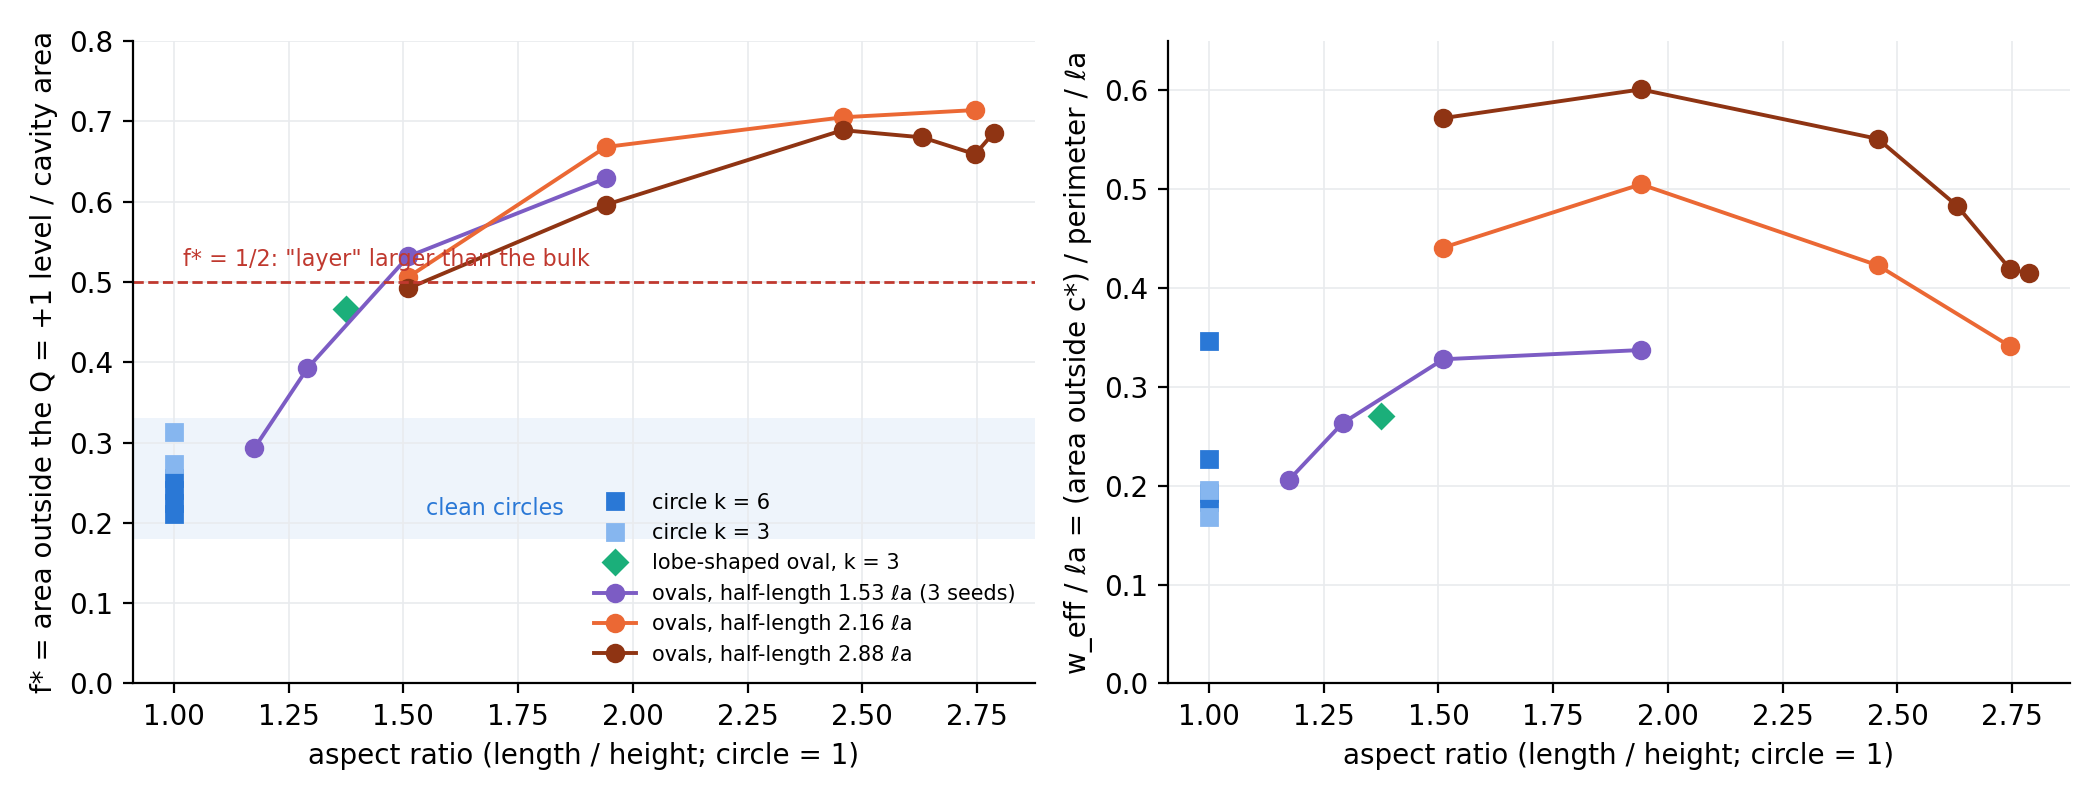
\includegraphics[width=\textwidth]{figs/layer_area.png}
\caption{Left: $f^*$ against the aspect ratio (length/height). Circles 0.20--0.32; ovals of all three sizes collapse onto
one curve (0.29 at aspect 1.17, crossing $\frac12$ near 1.5, levelling at 0.65--0.7); the lobe-shaped reference lies on it.
Right: $w_\mathrm{eff}/\la$, 0.17--0.25 for every clean circle layer, growing with size in ovals.}\label{fig:area}
\end{figure}
The collapse of $f^*$ against aspect ratio across sizes is itself the signature of ``no layer'', and identifies the
aspect ratio as the control parameter.

\subsection{Pinch-off: do the lobes become independent cavities?}
In the larger ovals $d^*$ falls again as the neck closes ($b/a\to1$). This is \textbf{not} a restored layer: in the
tightest necks ($b/a=1.01$--1.05) each lobe's charge passes $+1$ about 10 cells from the wall with slope
$\mathrm{d}Q/\mathrm{d}(c/b)\approx8$--10 (circle plateau $\approx3$), and the whole cavity passes $+2$ without a plateau.
Circles with the area of one lobe and half the winding ($k=3$, $R=23.9$ and $31.8$; server sweep, 3 seeds) keep a normal
layer ($d^*=4.1$--5.0 cells, plateau at $+1$). A lobe does not behave like a circle of its size.
\textbf{Lobe-shaped reference.} A single convex oval with the area and aspect of one lobe ($b/a=1.8$, half-length 30.4,
area 2171, aspect 1.38; $k=3$, 3 seeds) behaves like the pinched oval's lobes, not like the circle: only 3 pinned sites
(circle: $2k-2=4$), bulk $\approx1.9$ of 3, $d^*/\la=0.31$--0.32 (circles of the same area 0.18--0.22), no plateau, and
only 16--28\% of labelled wall defects at the wall after 1000 time units. \textbf{The lobe shape alone is enough to lose the
layer}; no coupling through the neck is needed. This matches the small-oval crossover: aspect 1.17 circle-like, 1.29
partial, $\ge1.38$ lost.


\subsection{Raising the winding in the pinched oval}
\begin{figure}[h]\centering
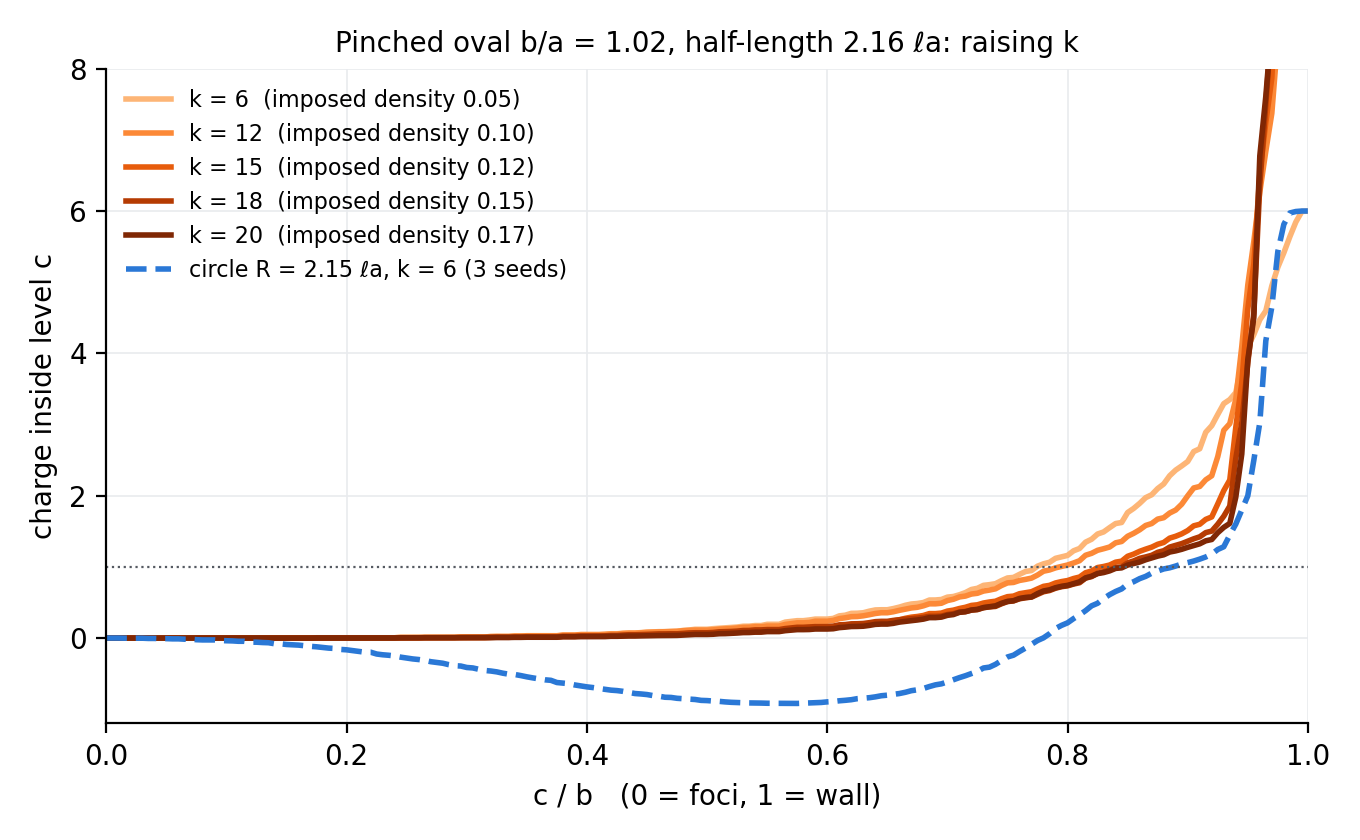
\includegraphics[width=0.82\textwidth]{figs/highk.png}
\caption{Accumulated charge in the pinched oval ($b/a=1.02$, half-length $2.16\,\la$) for $k=6$ to 20 (imposed density
0.05 to 0.17; the anchoring resolves up to $\approx0.15$), with the circle of $R=2.15\,\la$ for reference.}\label{fig:highk}
\end{figure}
A crowded wall partly restores the layer: the jump at the wall sharpens, $Q$ at $c/b=0.85$ falls from 1.76 ($k=6$) to
1.03--1.06 ($k=18$, 20), $d^*/\la$ from 0.38 to 0.30 (circle 0.20), and labelled wall defects stay at the wall (84\% after 1000
at $k=15$, 18). The bulk then carries $\approx+1$ \emph{for the whole cavity}, split as $\approx+\frac12$ per lobe, not $+1$
per lobe. So a high imposed defect density pushes the oval back towards the topological picture. $k=18$--20 is at the edge of
the anchoring resolution; 1 seed each.

\subsection{Activity $\zeta=0.09$ with three seeds}
$2k-2$ sites in all 27 runs, $q_b=1.01$--1.05, $P(q_b=+1)=0.77$--0.92, $\Phi=0.88$--0.99: the bulk charge is as clean as at
$0.07$, although the cavity centre is strongly depleted (Table~\ref{tab:dens}).
